\section{Finite conditional kernels and fresh multipliers}\label{sec:conditional}
We first construct the subspaces of finite codimension needed for the
midpoint estimates. The point is that conditioning on finitely many
coordinates has finite rank on the actual closed span $X_W$.

Independence and positivity give
\begin{equation}\label{prob:product-moments}
 \norm{P_v}=1,\qquad \E P_v^2=m_2^{|v|}.
\end{equation}
As a closed subspace of $L^1$, $X_W$ is a Banach space. The first-generation differences
$P_{(n)}-1=W_{(n)}-1$ are nonzero and pairwise orthogonal in $L^2$, so every
finite subset is linearly independent, also as elements of $L^1$.
Thus $X_W$ is infinite dimensional.
The first-generation products themselves are also linearly independent:
taking expectations in a relation $\sum_n a_nW_{(n)}=0$ gives
$\sum_n a_n=0$, reducing it to the corresponding relation among the
orthogonal differences. Rational finite combinations of the countable
family of products are dense, so $X_W$ is separable.

Let $T\subset\mathcal T$ be finite, contain the root, and contain every
predecessor of each of its vertices.  Write $\mathcal G_T$ for the
$\sigma$-field generated by the coordinates $W_v$ with
$v\in T\setminus\{\varnothing\}$.  For $v\in\mathcal T$, let $v_T$ be its
last ancestor in $T$.  Conditional expectation satisfies
\begin{equation}\label{prob:head-projection}
 Q_TP_v:=\E(P_v\mid\mathcal G_T)=P_{v_T}.
\end{equation}
Consequently $Q_T$ restricts to a contractive projection of $X_W$ onto the
finite-dimensional space
\[
 E_T=\operatorname{span}\{P_v:v\in T\},
 \qquad F_T=\ker(Q_T|_{X_W})\in\cof(X_W).
\]
This assertion on the completion follows from the continuity of conditional
expectation and the closedness of $E_T$.  Applying $I-Q_T$ to finite-product
approximations shows that finite-product combinations in $F_T$ are dense in
$F_T$.

The same space and tails can also be described using increments. Put
$u_v=P_v-P_{v^-}$ for $v\ne\varnothing$.  Telescoping along paths shows that
$\{1,u_v:v\ne\varnothing\}$ and $\{P_v:v\in\mathcal T\}$ have the same
algebraic span.  Formula~\eqref{prob:head-projection} gives $Q_Tu_v=u_v$
for $v\in T$ and $Q_Tu_v=0$ for $v\notin T$.  Applying $I-Q_T$ to the
algebraic span and then passing to its closure proves
\begin{equation}\label{prob:jump-tail}
 F_T=\overline{\operatorname{span}\{u_v:v\notin T\}}^{\,L^1}.
\end{equation}

For $t>0$ and $x,y\in X_W$, define the midpoint increment
\[
 M_t(x,y)=\frac{\norm{x+ty}+\norm{x-ty}}2-\norm{x}.
\]
The real scalar identity
$(|a+b|+|a-b|)/2=\max\{|a|,|b|\}$ gives
\begin{equation}\label{prob:midpoint-identity}
 M_t(x,y)=\E(t|y|-|x|)_+.
\end{equation}
For $u\in E_T$ and $y\in F_T$, we seek a lower bound on this excess in
terms of $\norm{y}$ and $\norm{u}$, uniform over $T$. Since $u$ is
$\mathcal G_T$-measurable, we first separate the fresh multipliers in $y$
from the coordinates determining $u$.

Now write a finite-product combination in the kernel as
$y=\sum_{v\in S}\alpha_vP_v\in F_T$, where $S\subset\mathcal T$ is finite.
Write $w\preceq v$ when $w$ is an ancestor of $v$, including $v$ itself,
and use $w\prec v$ for strict ancestry. Let $I$ be the finite set of first
vertices outside $T$ on paths to vertices of $S\setminus T$. Factoring out
the multiplier at each such exit gives
\[
 d=\sum_{v\in S\cap T}\alpha_vP_v,\qquad
 B_i=P_{i^-}\sum_{\substack{v\in S\\i\preceq v}}
       \alpha_v\prod_{i\prec w\preceq v}W_w\quad(i\in I),
\]
where an empty product is $1$. Thus $d$ is $\mathcal G_T$-measurable, and
$B_i$ depends only on old coordinates and on strict descendants of $i$,
not on $W_i$. Put $m_i=\E(B_i\mid\mathcal G_T)$. The factorization and
the condition $Q_Ty=0$ yield
\begin{equation}\label{prob:first-exit}
 y=d+\sum_{i\in I}W_iB_i,\qquad d=-\sum_{i\in I}m_i,
 \qquad \sigma=\Big(\sum_{i\in I}B_i^2\Big)^{1/2}.
\end{equation}
Distinct first-exit vertices have disjoint descendant subtrees.
Hence, conditionally on $\mathcal G_T$,
the $B_i$ are independent, and their entire vector is independent of the
first-exit variables $W_i$.  In particular, conditioning further on all
$B_i$ leaves the $W_i$ independent with their original law.  Write
\[
 \mathcal H_T=\mathcal G_T\vee\sigma(B_i:i).
\]
We will condition on $\mathcal G_T$ when copying entire coefficients, and
on $\mathcal H_T$ when resampling only first-exit multipliers. Figure~\ref{fig:exit}
illustrates this distinction. All quantities
used here are integrable; in fact the finite products belong to $L^2$.

\begin{figure}[ht]
\centering
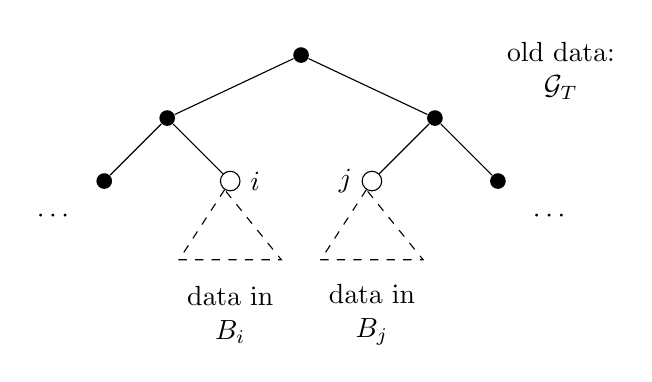
\begin{tikzpicture}[x=1cm,y=1cm,
 old/.style={circle,fill=black,inner sep=2pt},
 fresh/.style={circle,draw,fill=white,inner sep=2.5pt}]
 \node[old,label=above:{$\varnothing$}] (r) at (0,1.6) {};
 \node[old] (a) at (-1.7,.8) {};
 \node[old] (b) at (1.7,.8) {};
 \node[old] (a1) at (-2.5,0) {};
 \node[fresh,label=right:{$i$}] (i) at (-.9,0) {};
 \node[fresh,label=left:{$j$}] (j) at (.9,0) {};
 \node[old] (b1) at (2.5,0) {};
 \draw (r)--(a)--(a1) (a)--(i) (r)--(b)--(j) (b)--(b1);
 \draw[dashed] (i)--(-1.55,-1)--(-.25,-1)--cycle;
 \draw[dashed] (j)--(.25,-1)--(1.55,-1)--cycle;
 \node[align=center] at (-.9,-1.7) {data in\\$B_i$};
 \node[align=center] at (.9,-1.7) {data in\\$B_j$};
 \node[align=center] at (3.3,1.4) {old data:\\$\mathcal G_T$};
 \node at (-3.15,-.45) {$\cdots$};
 \node at (3.15,-.45) {$\cdots$};
\end{tikzpicture}

\caption{A finite predecessor-closed set $T$ (solid vertices) and two first-exit
vertices $i,j$ (open vertices). Only $W_i,W_j$ are resampled after the
coefficients $B_i,B_j$ have been fixed. Those coefficients may depend on the
old coordinates and on the disjoint strict descendant subtrees (triangles).
Only finitely many exits occur in a finite linear combination; the ambient tree
has countably many children at every vertex.}\label{fig:exit}
\end{figure}

The next two estimates measure the size of a tail vector by the expected
Euclidean size of its coefficient list. Their upper bounds on $\norm{y}$
give lower bounds on $\E\sigma$, which the scalar estimates in
Sections~\ref{sec:exponential} and~\ref{sec:gaussian} will convert into
midpoint gains. They use independent-copy
symmetrization followed by averaging over independent signs; this is the
standard symmetrization method, here applied conditionally on the old
coordinates \cite[proof of Theorem~8, p.~468]{BartlettMendelson2002}.
Both constants will be useful: they come from different ways of centering
the sum.
\begin{lemma}[Two first-moment estimates]\label{prob:first-moment}
For the representation~\eqref{prob:first-exit},
\begin{align}
 \norm{y}&\le\bigl(\sqrt{m_2-1}+2\bigr)\E\sigma,
 \label{prob:first-moment-centered}\\
 \norm{y}&\le2\sqrt{m_2}\,\E\sigma.
 \label{prob:first-moment-signed}
\end{align}
Both inequalities also hold conditionally on $\mathcal G_T$, with
$\E(|y|\mid\mathcal G_T)$ and $\E(\sigma\mid\mathcal G_T)$ in place
of the unconditional first moments.
\end{lemma}
\begin{proof}
Work conditionally on $\mathcal G_T$, suppressing this conditioning in the
expectation notation throughout the proof. Integrating the resulting
inequalities gives the unconditional statements.
First write
\[
 y=\sum_iB_i(W_i-1)+\sum_i(B_i-m_i).
\]
After fixing all $B_i$, the first sum has mean zero
and second moment $(m_2-1)\sigma^2$.  Its expected absolute value is thus
at most $\sqrt{m_2-1}\,\E\sigma$ after averaging over the $B_i$.
For the second sum, take independent copies $B_i'$ of the independent
$B_i$. Jensen's inequality,
independent random signs $\varepsilon_i$, and Cauchy--Schwarz give
\begin{align*}
 \E\Big|\sum_i(B_i-m_i)\Big|
 &\le\E\Big|\sum_i(B_i-B_i')\Big|\\
 &=\E\E_{\varepsilon}\Big|\sum_i\varepsilon_i(B_i-B_i')\Big|\\
 &\le\E\Big(\sum_i(B_i-B_i')^2\Big)^{1/2}
 \le2\E\sigma.
\end{align*}
The equality uses independence and symmetry of the differences. Combining
the two estimates proves~\eqref{prob:first-moment-centered} conditionally.

For the other estimate, put
$U_i=W_iB_i$.  These variables are independent, and $y=\sum_i(U_i-\E U_i)$.
Symmetrizing with independent copies $U_i'$ and inserting independent signs
as above yields
\begin{align*}
 \E|y|
 &\le\E\E_{\varepsilon}\Big|\sum_i\varepsilon_i(U_i-U_i')\Big|\\
 &\le2\E\E_{\varepsilon}\Big|\sum_i\varepsilon_iU_i\Big|
 \le2\E\Big(\sum_iW_i^2B_i^2\Big)^{1/2}.
\end{align*}
With the $B_i$ fixed, concavity of the square root bounds the expectation
over the $W_i$ of $\bigl(\sum_iW_i^2B_i^2\bigr)^{1/2}$ by
$\sqrt{m_2}\,\sigma$. Averaging over the $B_i$ proves
\eqref{prob:first-moment-signed} conditionally on $\mathcal G_T$.
\end{proof}

The preceding construction applies to finite-product tails. To pass
midpoint estimates to their closure, the triangle inequality gives
\begin{equation}\label{prob:continuity}
 |M_t(x,y)-M_t(x',y')|
 \le2\norm{x-x'}+t\norm{y-y'}.
\end{equation}
Thus all tail estimates below pass to the completed tail subspace before
we impose the condition $\norm{y}\ge1$.


\begin{lemma}[Passage to completed tails and arbitrary centers]\label{lem:affine}
Fix $t>0$ and nonnegative constants $A,B$. Suppose that, for every finite
predecessor-closed $T$, every $u\in E_T$, and every finite-product
combination $y\in F_T$,
\[
 M_t(u,y)\ge A\norm{y}-B\norm{u}.
\]
Then this inequality holds for all $y\in F_T$, and
\[
 \whdelta_{X_W}(t)\ge\max\{0,A-B\}.
\]
\end{lemma}
\begin{proof}
The first assertion follows from density in $F_T$ and
\eqref{prob:continuity}. For a unit vector $x$ and any $\varepsilon>0$,
choose a finite-product combination $u$ with $\norm{x-u}<\varepsilon$,
and let $T$ contain the root and all its support paths. Then $u\in E_T$,
$\norm{u}\le1+\varepsilon$, and every $y\in F_T$ with $\norm{y}\ge1$
satisfies
\[
 M_t(x,y)\ge A-B-(B+2)\varepsilon.
\]
For this fixed $x$, take the supremum over finite-codimensional subspaces
and let $\varepsilon\downarrow0$. The resulting bound $A-B$ is independent
of $x$, so it survives the final infimum. The scalar midpoint identity
also gives the lower bound zero.
\end{proof}

The lemma is applied to norm inequalities, not to an infinite first-exit
expansion. Thus no representation or extra integrability of a general
completed tail is needed. It also fixes the order of choices: $t$ and
$x$ determine $T$ before the direction $y$ is allowed to vary.
